\documentclass{beamer}
\mode<presentation>{
    \usetheme{Antibes}
    \usecolortheme{lily}
    \setbeamertemplate{footline}[frame number] % To replace the footer line in all slides with a simple slide count
    \setbeamertemplate{navigation symbols}{} % To remove the navigation symbols from the bottom of all slides
}
\usepackage[utf8]{inputenc}
\usepackage[T1]{fontenc}
\usepackage[francais]{babel}
\usepackage{graphicx}
\usepackage{tikz}
\usepackage{hyperref}

\title[Thibault Vanwersch -- Présentation du master en security]{Université Libre de Bruxelles :\\
Master in Cybersecurity}

\author{Thibault Vanwersch}
\institute{\href{mailto:thibault@vanwersch.fr}{thibault@vanwersch.fr}}
\date{08 décembre 2017}

\begin{document}
\begin{frame}
    \titlepage
\end{frame}

\section{Introduction}

\begin{frame}[c]
  \frametitle{Le master}
    Union de 4 universités et 2 hautes école\only<2->{ : 1 diplôme}
  \begin{figure}
    
\includegraphics[width=\textwidth]{imgs/4university.png}
  \end{figure}
\end{frame}

{ % all template changes are local to this group.
    \setbeamertemplate{navigation symbols}{}
    \setbeamercolor{background canvas}{bg=black}
    \begin{frame}[plain]
        \begin{tikzpicture}[remember picture,overlay]
            \node[at=(current page.center)] {
                
\includegraphics[width=\paperwidth]{imgs/iliketrain.jpg}
            };
        \end{tikzpicture}
     \end{frame}
}

\section{Contenu}

\begin{frame}[c]
  \begin{figure}
    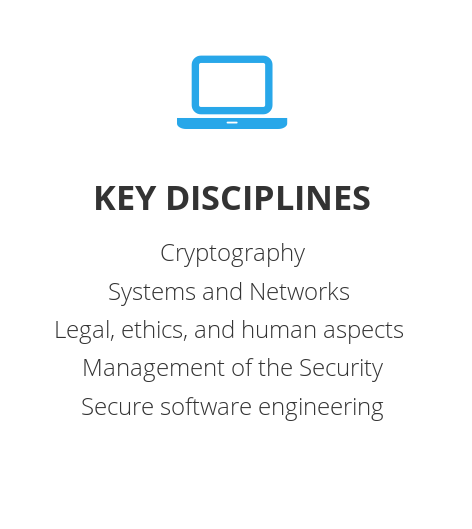
\includegraphics[height=\textheight]{imgs/key_disciplines.png}
  \end{figure}
\end{frame}

\begin{frame}[c]
  \begin{figure}
    
\includegraphics[height=\textheight]{imgs/projects_challenges.png}
  \end{figure}
\end{frame}

\subsection{Passerelle}
\begin{frame}[c]
  \frametitle{Passerelle}

    \begin{description}[align=left,labelwidth=\textwidth]
        \item[PROJ-H415] Project Electronics and Telecommunication
        \item[MATH-F307] Mathématiques discrètes
        \item[INFO-F302] Informatique fondamentale
        \item[INFO-Y561] Organisation et gestion des entreprises
        \item[INFO-Y560] Communication anglophone contextualisée
        \item[INFO-Y555] Télécommunications et réseaux
        \item[INFO-Y554] Probabilités et statistiques
        \item[INFO-Y553] Computability and complexity
        \item[ELEC-H310] Digital electronics
        \item[TRAN-H3001] De l'épistémologie des sciences à la gestion de projet
        \item[MATH-H2002] Calcul des probabilités et statistiques
        \item<2->[INFO-F405] \textcolor{gray}{Introduction to cryptography}
        \item<2->[INFO-Y115] \textcolor{gray}{Secure software design and web security}
        \item<2->[INFO-Y111] \textcolor{gray}{Computer system security}
    \end{description}
\end{frame}

\subsection{1ère année}
\begin{frame}[c]
  \frametitle{1ère année}
  \begin{figure}
    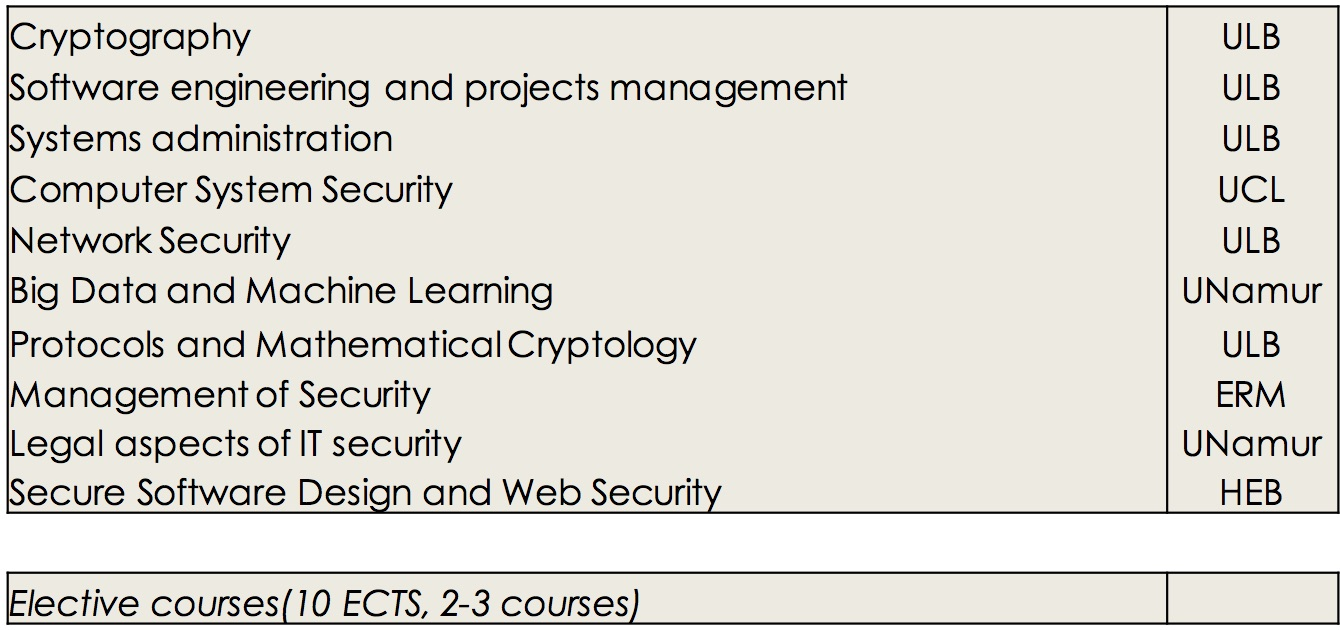
\includegraphics[width=\textwidth]{imgs/cursus1.jpg}
  \end{figure}
\end{frame}

\subsection{2ème année}
\begin{frame}[c]
  \frametitle{2ème année}
  \begin{figure}
    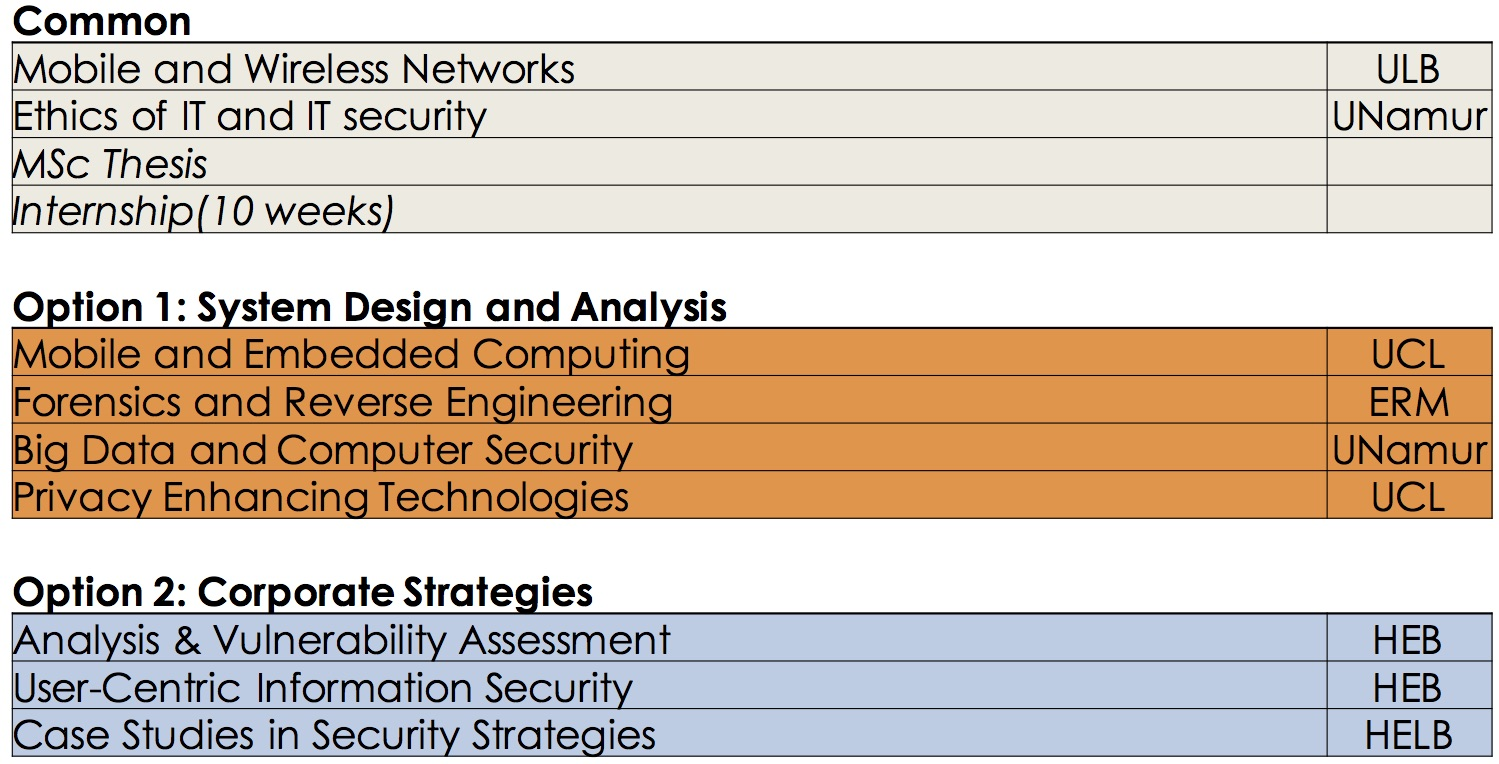
\includegraphics[width=\textwidth]{imgs/cursus2.jpg}
  \end{figure}
\end{frame}

\section{Débouchés}
\begin{frame}[c]
  \frametitle{Débouchés}
    \par Plein de domaines :
    \begin{itemize}
        \item Grosses entreprises avec de l'informatique
        \item Industrie du logiciel
        \item Télécommunication
        \item Administration publique
        \item Armée
        \item Forces de l'ordre
        \item Banques
        \item (...)
    \end{itemize}
\end{frame}

\begin{frame}[c]
    \par Typiquement, on retrouve des experts en cybersécurité aux postes suivant :
    \begin{itemize}
        \item Security Officer
        \item Computer emergency response team member (CERT)
        \item Forensics expert
        \item Security architect
        \item Network architect
        \item Security analyst, consultant and/or auditor
        \item Researchers
    \end{itemize}
\end{frame}

\section{Ressources}
\begin{frame}[c]
    \frametitle{Ressources :}
    \begin{itemize}
        \item \url{https://masterincybersecurity.ulb.ac.be/}
        \item \url{https://masterincybersecurity.ulb.ac.be/students/}
        \item \url{http://banssbfr.ulb.ac.be/PROD\_frFR/bzscrse.p\_disp\_prog\_detail?term\_in=201718\&prog\_in=MA-SECU\&lang=AMERICAN}
        \item \url{https://github.com/thibault-v/slides\_msecuc\_ipl}
    \end{itemize}
\end{frame}

%------------------------------------------------
\section{Question}

\begin{frame}
    \centerline{\Huge{Question ?}}
    \vspace*{30px}
    \centerline{\href{mailto:thibault@vanwersch.fr}{thibault@vanwersch.fr}}
    \vspace*{10px}
    \centerline{\tt PGP fingerprint : EA36 73B0}
\end{frame}
%----------------------------------------------------------------------------------------
\end{document}
